
\chapter{Contribution}\label{chap:contribution}
The goal of this thesis is to analyze the relationship between selfish mining and networking effects. Therefore, the model proposed by \gopalan has been enhanced to model selfish mining behaviour in \ref{selfishmodel}. The main contributions are based on simulative evaluations and can be categorized as the following:
\begin{enumerate}
	\item Implementation and Verification of Blockchain Gossip Model~\cite{gopalan}
	\item Integration of selfish mining as described in \ref{selfishmodel} in Blockchain Gossip Model 
	\item Analysis of networking characteristics
	\item Analysis of selfish mining characteristics
	\item Model verification
\end{enumerate}
Contributions are building blocks for each other. Integration of selfish mining is only possible when the Blockchain Gossip Model has been implemented.
As such the following sections will discuss contributions in a developing and chronological order.

\section{Implementation and Verification of Blockchain Gossip Model}

The core implementation of the Blockchain Gossip Model Simulator is based on simpy~\cite{simpy}. Simpy is a process based discrete event simulator. The Blockchain Gossip Model described by \citeauthor{gopalan}~\cite{gopalan} consists of four parts. 
\begin{itemize}
\item Networkgraph representation
\item Blockchain representation
\item Block Arrival Process representation
\item Communication Process representation
\end{itemize}
\paragraph{Parameter Setup}
The network graph is represented by an adjacency matrix. In the synthetic data experiments of \gopalan  they analyze the complete graph for 10, 20 and 30 peers. There the matrix representing the network graph is an unit matrix.
The blockchain representation is a set of blocks and a set of edges for each peer, which are developing over time.
The block arrival process and the communication process are modelled as a poisson process. Specifically to a discrete event simulator, this implies that the interarrival time between scheduled events follows an exponential distribution. On each event of the block arrival process a block arrives uniformly at a random peer. At each event of the communication process $T_i$ a peer $p_i$ tries to update a certain peer $p_j$ according to the epoch associated with the event.
The block to be updated is deterministically chosen. According to \gopalan the block with the lowest index number is chosen. Additionally, the average rate of the communication processes is set to one.

\paragraph{Evaluation of Simpy Blockchain Simulator on synthetic data experiments}
\citeauthor{gopalan} introduce four key metrics to analyze the system. Those are 
\begin{itemize}
\item Time to Consistency --- The average time an inconsistent system needs to reach a state of consistency
\item Cycle Length --- The sum of the average time to consistency and the average of the time the system stays consistent
\item Consistency Fraction --- The average fraction of peers that are consistent at each point in time
\item Age of Information --- The average number of blocks an average peer is away from the consistency state
\end{itemize}
All metrics mentioned above refer to the term consistency. \gopalan define consistency as $B(t)$~\ref{unisondef}, the unison of all blocks produced by the block arrival process $A$.
These metrics can be used to verify whether the Simpy Blockchain Gossip Model Simulator is achieving similar numbers to the implementation of \gopalan . 
\begin{figure}[h]
	\begin{subfigure}[b]{0.48\textwidth}
		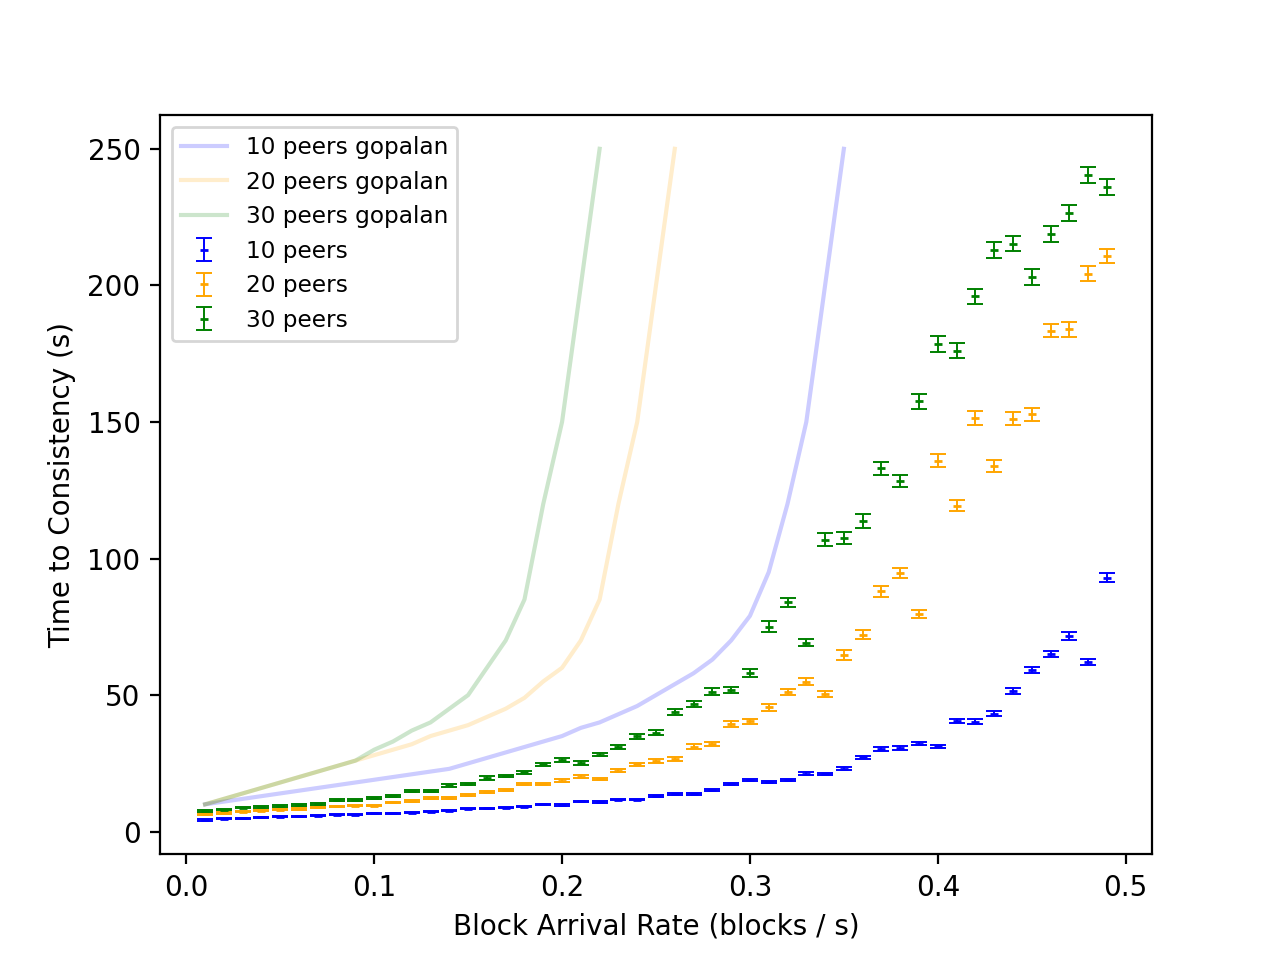
\includegraphics[width=\textwidth]{figures/gopalan_figures/time_to_consistency.png}
		\caption{ Time to Consistency, Comparison between Blockchain Gossip Model Simulator based on simpy and values produced by \gopalan}
		\label{fig:gopalan_ttc}
	\end{subfigure}
	\hfill
	\begin{subfigure}[b]{0.48\textwidth}
		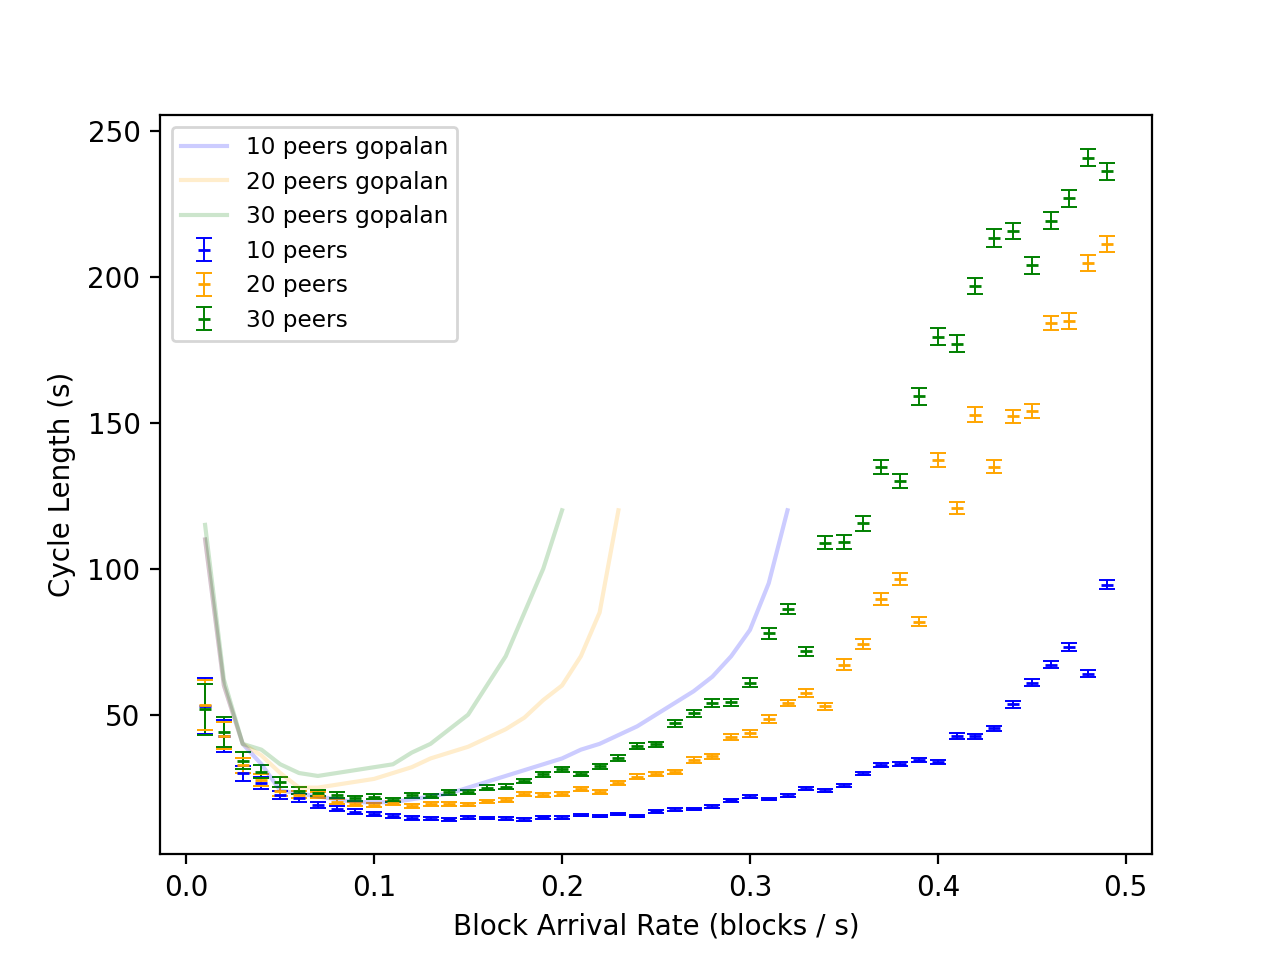
\includegraphics[width=\textwidth]{figures/gopalan_figures/cycle_length_avg.png}
		\caption{ Cycle Length, Comparison between Blockchain Gossip Model Simulator based on simpy and values produced by \gopalan}
		\label{fig:gopalan_cl}
	\end{subfigure}
	\hfill
	\begin{subfigure}[b]{0.48\textwidth}
		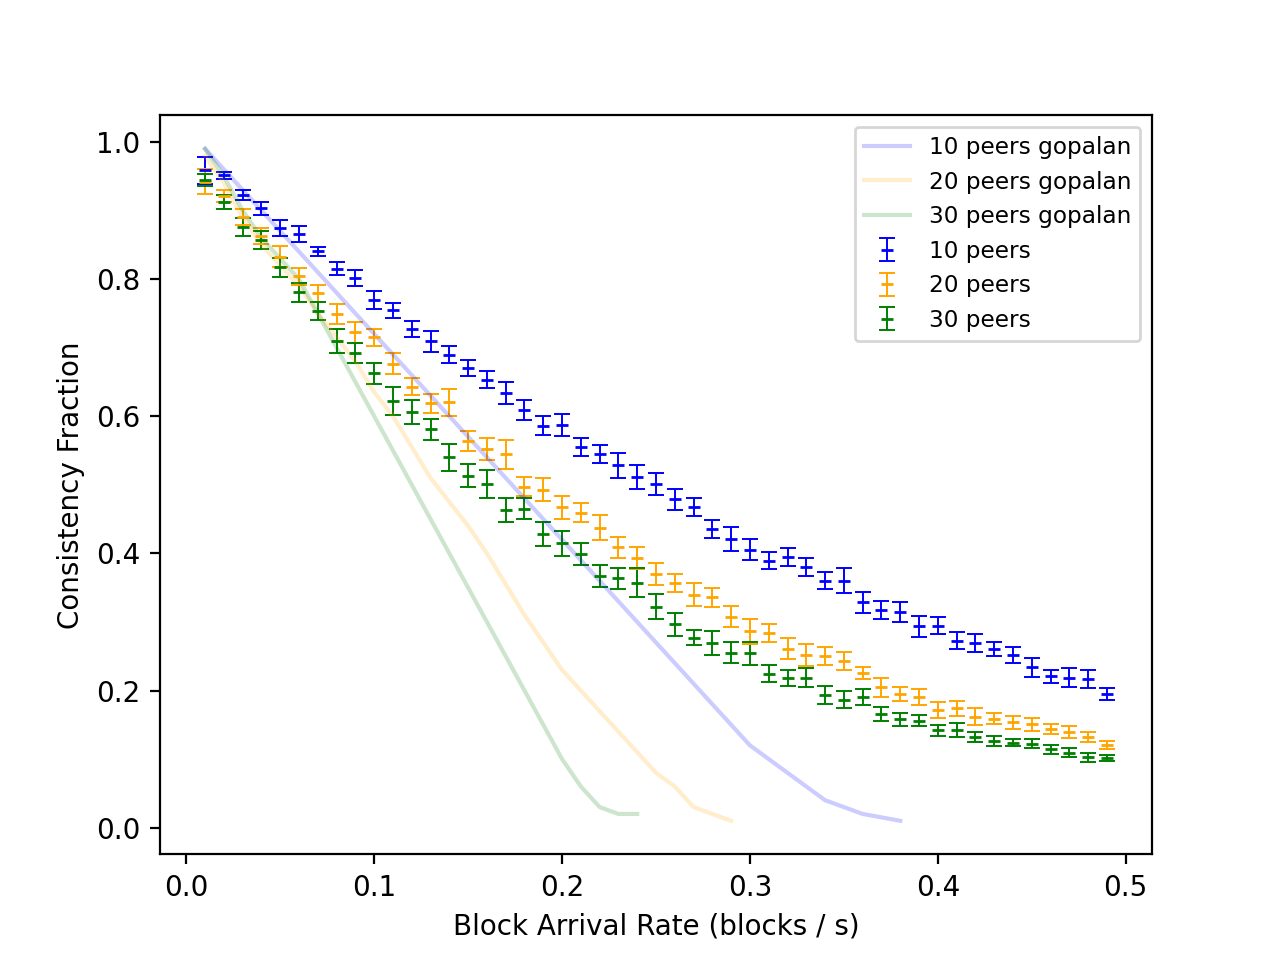
\includegraphics[width=\textwidth]{figures/gopalan_figures/consistency_fraction.png}
		\caption{ Consistency Fraction, Comparison between Blockchain Gossip Model Simulator based on simpy and values produced by \gopalan}
		\label{fig:gopalan_cf}
	\end{subfigure}
	\hfill
	\begin{subfigure}[b]{0.48\textwidth}
		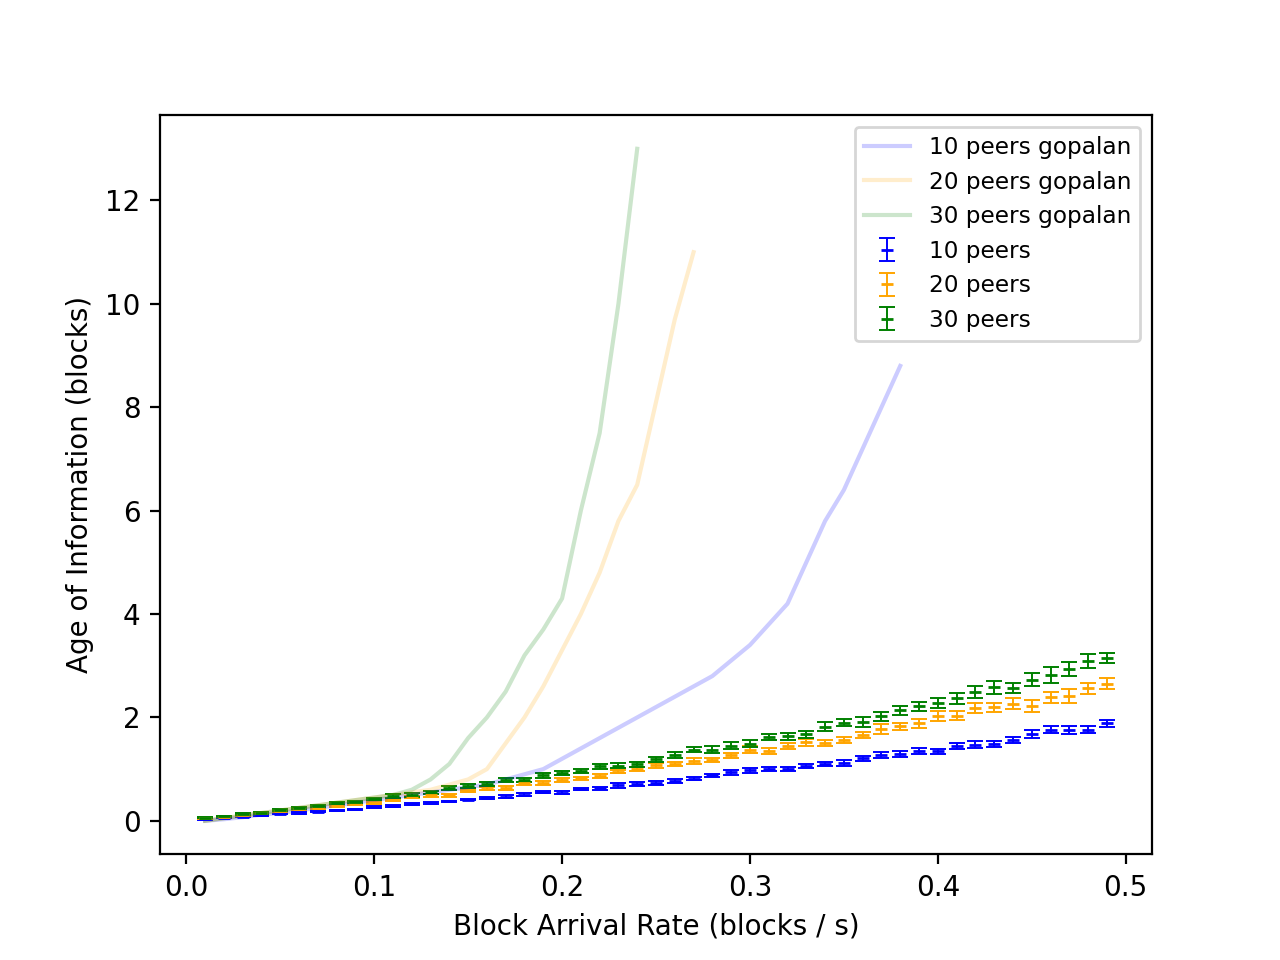
\includegraphics[width=\textwidth]{figures/gopalan_figures/age_of_information.png}
		\caption{ Age of Information, Comparison between Blockchain Gossip Model Simulator based on simpy and values produced by \gopalan}
		\label{fig:gopalan_aof}
	\end{subfigure}
\end{figure} 

The metrics of time to consistency and cycle length are very closely related, because both rely on the time the system needs to reach consistency.
Figure~\ref{fig:gopalan_ttc} and Figure~\ref{fig:gopalan_cl} show this close relationship. Additionally the comparison between the simpy version of the Blockchain Gossip Model Simulator shows a very similar tendency in both metrics. Especially in Figure~\ref{fig:gopalan_ttc} it is observable that the curve has the same tendency, but has a flatter increase when the Block Arrival Rate increases. Figure~\ref{fig:gopalan_ttc} shows that an increase in number of peers or an increasing Block Arrival Rate leads to an increase in the average Time to Consistency. Since Cycle Length is the sum of the average time to consistency and the average of the time the system stays consistent the same behavior can be observed in Figure~\ref{fig:gopalan_cl}. Additionally Figure~\ref{fig:gopalan_cl} shows that for very small numbers for the Block Arrival Rate the cycle length increases again. When the system has a low Block Arrival Rate the system tends to stay longer in a state of consistency, the idle time increases.

Consistency fraction and age of information are both metrics measuring the consistency of an average peer. The consistency fraction is the fraction of peers, which have a blockset equal to $B(t)$~\ref{unisondef}. For both the simulation results by \gopalan and the simpy version of the Blockchain Gossip Model Simulator we can observe, that the consistency fraction decreases with an increasing blockrate and peer number. While the exact numbers do differ, similar tendencies can again be observed.
The age of information metric analysis how much an average peer differs from $B(t)$~\ref{unisondef}. It showcases an increase for an increasing blockrate and peer number.

The differences between the simulation results by \gopalan and the simpy version of the Blockchain Gossip Model Simulator indicate that information spreads faster in the simpy version of the Blockchain Gossip Model Simulator. This is most probably due to the fact that the implemented communication processes are truly concurrent.	


%The relationship between selfish mining and networking effects can be charactized by a number of key questions.
%Those questions can be split up in two groups.
%The first group considers how the network influences selfish mining.
%Key aspects include:
%begin{enumerate}
%\item \citet{xiao_modeling} show in their model that revenue gain and profitability threshhold correlates to betweenness centrality. Does this correlation also show \ref{selfishmodel}?
%\item Does a networking advantage increase revenue gain and profitability threshhold?
%\item Does a certain network topology influence selfish mining effectiveness?
%\end{enumerate}
%The second group considers how selfish mining influences the network.
%Key aspects include:
%\begin{enumerate}
%\item Does the network have a different throughput, if one peer is executing the selfish mining protocol?
%\item Does the network have a different block propagation time, if one peer is executing the selfish mining protocol?
%\item Does the network show different congestion peeks, if one peer is executing the selfish mining protocol?
%\item If the network shows congestion peeks, does it correlate to certain actions the selfish miner is performing?
%\end{enumerate}
%´%


\section{gopalan modell extension}
%- pre selfish mining\\
%- blockchain \\ metriken umdefinieren sodass sie auf bäumen funktionieren 
%- addit. network metrics, block propagation etc.
%- consensus  \\ umdefinieren
%- grpahen? falls es lohnt, falls unterschied auftritt, falls alles sehr gleich, das halt auch besprechen

\section{selfish mining extension}
%selfish mining in modell rein,
%metriken zu selfish mining
%graphen, diskussion etc.







